\documentclass[tikz,border=3pt]{standalone}
\usepackage{tikz}
\usetikzlibrary{positioning,arrows.meta,fit,backgrounds,calc,decorations.pathmorphing}
\usepackage[scaled]{helvet}
\usepackage{amsmath,amssymb}
\renewcommand{\familydefault}{\sfdefault}
\definecolor{qnt}{HTML}{6C3FA0}
\definecolor{qntl}{HTML}{ECE3F6}
\definecolor{mal}{HTML}{C0392B}
\definecolor{mall}{HTML}{F8DEDB}
\definecolor{mec}{HTML}{1E8449}
\definecolor{grey}{HTML}{5D6D7E}
\tikzset{
  blk/.style={rectangle, rounded corners=2pt, draw, thick, align=center, font=\scriptsize, inner sep=2.5pt},
  bs/.style={rectangle, draw=black, fill=gray!25, minimum width=3.2mm, minimum height=3.2mm, rotate=45, inner sep=0pt},
  det/.style={shape=rectangle, draw, fill=black!75, minimum width=2.4mm, minimum height=3.2mm, inner sep=0},
  opt/.style={qnt, line width=1.1pt},
  arr/.style={-{Stealth[length=1.6mm]}, thick},
  lab/.style={font=\tiny, align=center},
}
\begin{document}
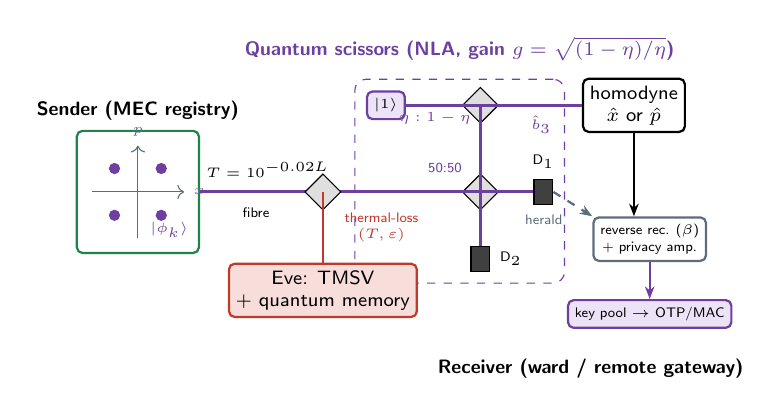
\begin{tikzpicture}[x=1cm,y=1cm]
% Alice (MEC trust registry)
\node[blk, draw=mec, minimum width=1.55cm, minimum height=1.55cm] (A) at (-0.15,0) {};
\node[font=\scriptsize\bfseries, anchor=south] at (A.north) {Sender (MEC registry)};
% QPSK constellation inside
\begin{scope}[shift={(A.center)}, scale=0.42]
\draw[->, grey] (-1.4,0) -- (1.4,0) node[right, font=\tiny]{$x$};
\draw[->, grey] (0,-1.4) -- (0,1.4) node[above, font=\tiny]{$p$};
\foreach \k in {0,1,2,3} {\fill[qnt] ({cos(45+90*\k)},{sin(45+90*\k)}) circle (0.17);}
\node[font=\tiny, text=qnt] at (0.95,-1.15) {$|\phi_k\rangle$};
\end{scope}
% channel
\coordinate (c0) at (A.east);
\coordinate (c1) at (3.3,0);
\draw[opt] (c0) -- (c1);
\node[lab, below] at (1.35,-0.08) {fibre};
\node[lab, above] at (1.5,0.06) {$T=10^{-0.02L}$};
% Eve entangling cloner
\node[bs] (bsE) at (2.2,0) {};
\node[blk, draw=mal, fill=mall, minimum width=1.4cm] (E) at (2.2,-1.25) {Eve: TMSV\\ + quantum memory};
\draw[mal, thick] (E.north) -- (bsE.center);
\node[lab, text=mal, anchor=west] at (2.35,-0.45) {thermal-loss\\ $(T,\varepsilon)$};
% Bob: quantum scissors
\node[bs] (bs2) at (4.2,0) {};
\node[bs] (bs1) at (4.2,1.1) {};
\node[blk, draw=qnt, fill=qntl, font=\tiny] (ph) at (3.0,1.1) {$|1\rangle$};
\draw[opt] (c1) -- (bs2.center);
\draw[opt] (ph.east) -- (bs1.center);
\node[lab, text=qnt] at (3.62,0.93) {$\eta:1-\eta$};
\draw[opt] (bs1.center) -- (bs2.center);
\node[det] (D1) at (5.0,0) {};
\node[det] (D2) at (4.2,-0.85) {};
\draw[opt] (bs2.center) -- (D1.west);
\draw[opt] (bs2.center) -- (D2.north);
\node[lab, above] at (D1.north) {D$_1$};
\node[lab, right] at (D2.east) {D$_2$};
\node[lab, text=qnt] at (3.75,0.3) {50:50};
% output to homodyne
\node[blk, draw=black, minimum width=1.25cm] (hd) at (6.15,1.1) {homodyne\\ $\hat x$ or $\hat p$};
\draw[opt] (bs1.center) -- (hd.west) node[pos=0.6, below, lab]{$\hat b_3$};
\node[blk, draw=grey, minimum width=1.4cm, font=\tiny] (pp) at (6.35,-0.6) {reverse rec. ($\beta$)\\ + privacy amp.};
\draw[arr] (hd.south) -- (hd.south |- pp.north);
\draw[arr, grey, dashed] (D1.east) -- node[below left, lab]{herald} (pp.north west);
\node[blk, draw=qnt, fill=qntl, font=\tiny] (kp) at (6.35,-1.55) {key pool $\to$ OTP/MAC};
\draw[arr, qnt] (pp) -- (kp);
\begin{scope}[on background layer]
\node[rounded corners=4pt, draw=qnt, dashed, fit=(ph)(bs1)(bs2)(D1)(D2), inner sep=4pt,
 label={[font=\scriptsize\bfseries, text=qnt, yshift=1mm]above:Quantum scissors (NLA, gain $g=\sqrt{(1-\eta)/\eta}$)}] {};
\end{scope}
\node[font=\scriptsize\bfseries, anchor=north] at (5.6,-2.0) {Receiver (ward / remote gateway)};
\end{tikzpicture}
\end{document}
